\documentclass{article}
\usepackage{graphicx} 

\title{Problem Set 6}
\author{Todvwa Dlamini  \\ Econ 5253}
\date{March 24 2026}

\begin{document}
\maketitle

\section{Data Cleaning}
The original dataset contained two rows of column labels, so I removed the first row and used the second row as the proper column names. I then renamed the variables to more concise and readable names: \texttt{country\_or\_territory}, \texttt{est\_lang}, \texttt{imm\_lang}, \texttt{total\_lang}, \texttt{world\_lang\_pct}, \texttt{total\_speakers}, \texttt{mean\_speakers}, and \texttt{median\_speakers}.

Additionally, several variables were initially stored as character strings due to formatting issues such as spaces and other non-numeric characters. I cleaned these variables by removing non-numeric characters and converting them into numeric format. All variables were converted to numeric except for \texttt{country\_or\_territory}, which remained as a character variable since it represents categorical information. 

\section{Data Visualization}

Three visualizations were created to explore patterns in linguistic diversity and language distribution across countries.

\subsection{Top 10 Most Linguistically Diverse Countries}

\begin{figure}[h!]
\centering
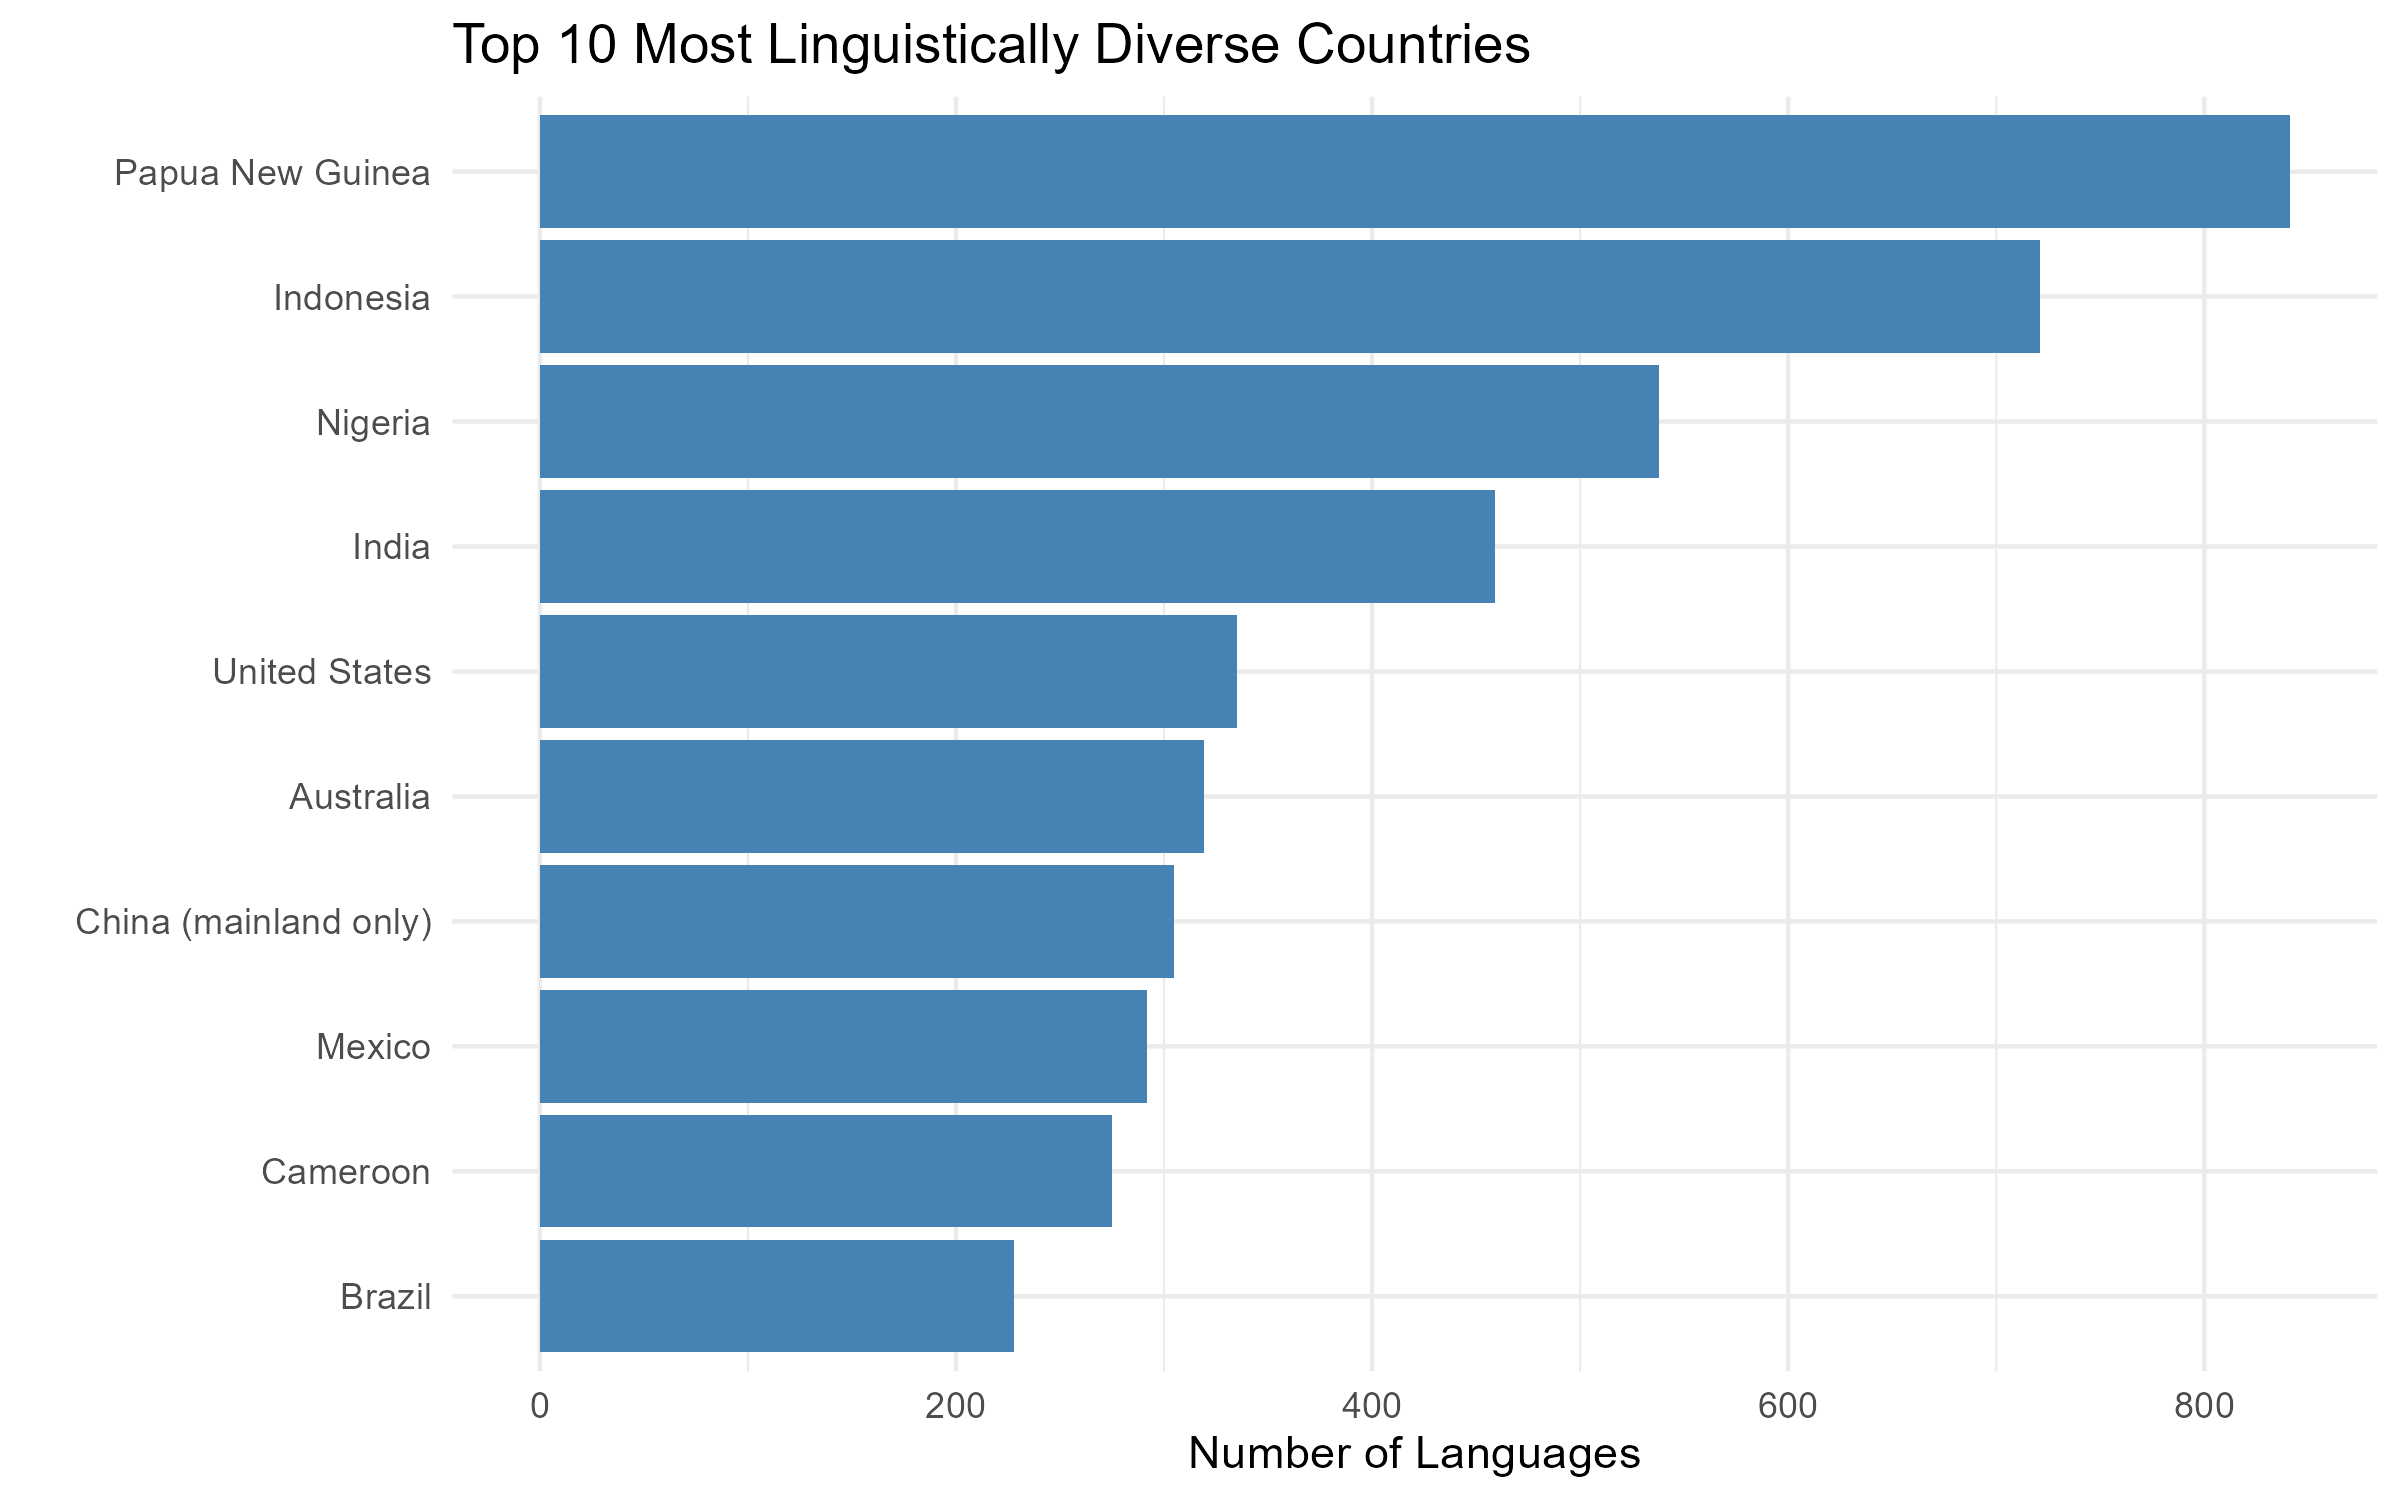
\includegraphics[width=0.8\textwidth]{PS6a_Dlamini.png}
\caption{Top 10 countries by number of languages}
\end{figure}
This bar chart shows the 10 most linguistically diverse countries. It demonstrates that the linguistic diversity is greatly localized in few countries, with Papua New Guinea, Indonesia and Nigeria possessing much higher number of languages than any other countries. This can help us understand that the linguistic diversity of the world is not uniformly distributed over the globe, but rather concentrated in certain areas.



\subsection{Linguistic Diversity and Language Size}

\begin{figure}[h!]
\centering
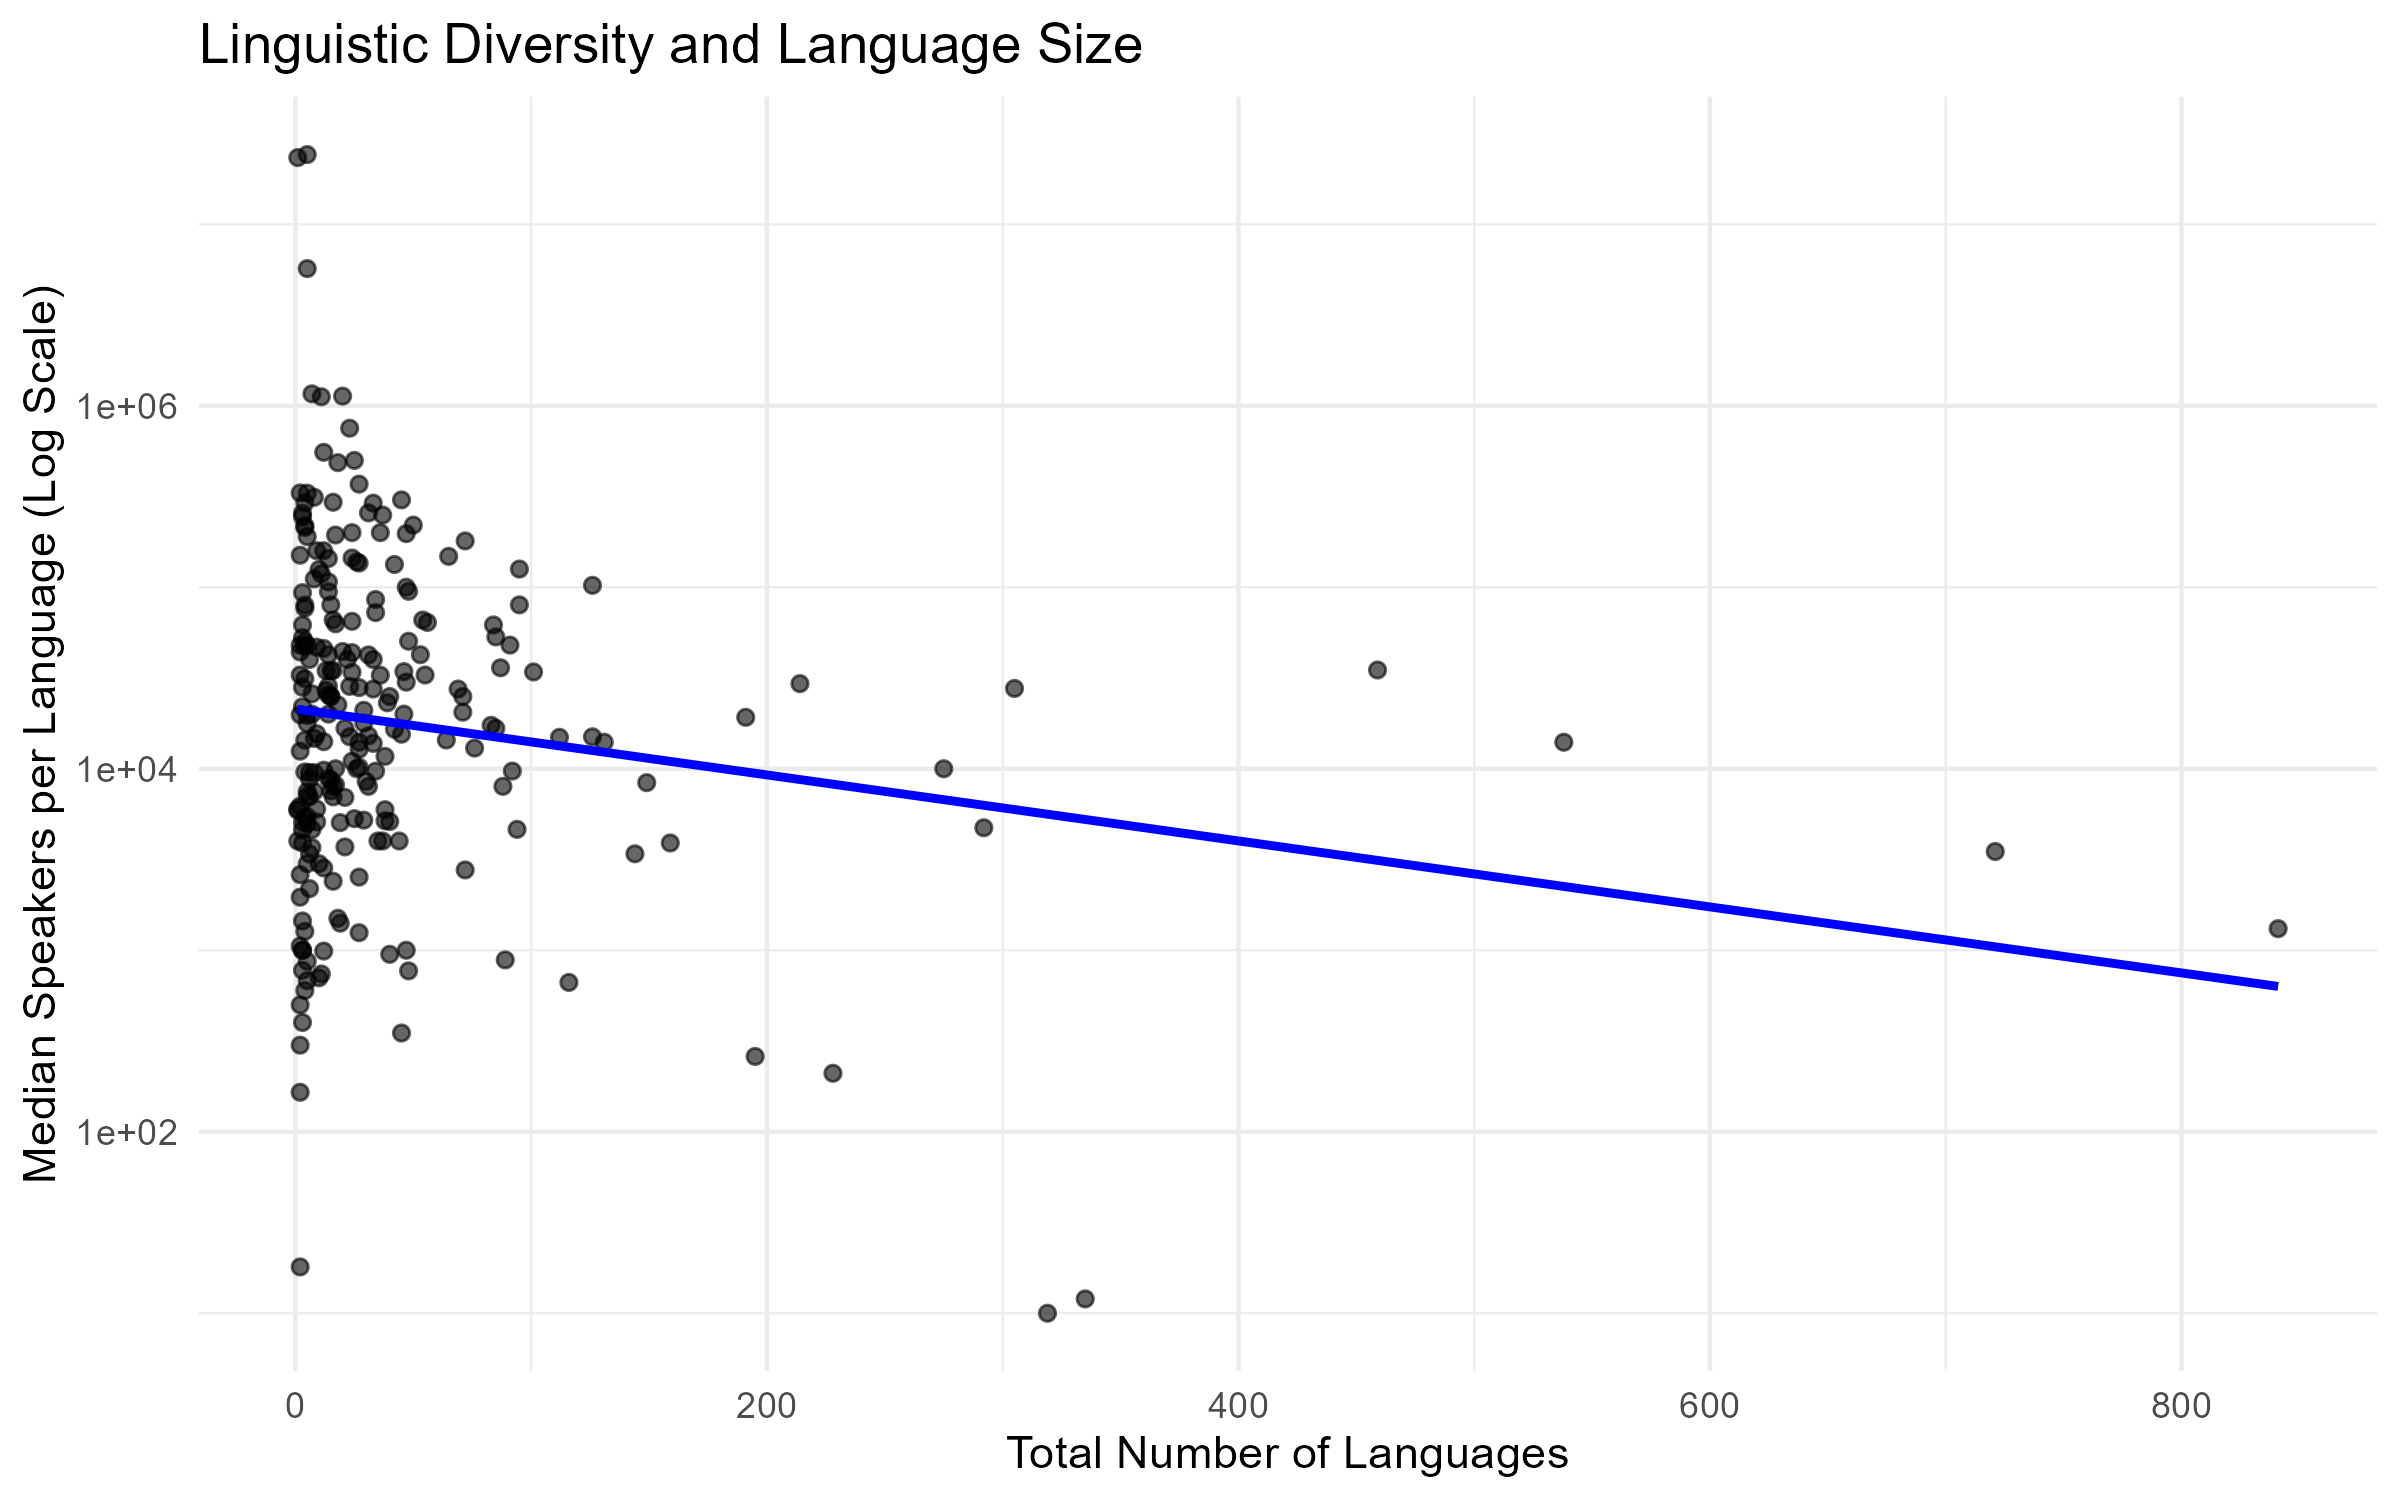
\includegraphics[width=0.8\textwidth]{PS6b_Dlamini.png}
\caption{Relationship between number of languages and median number of speakers per language}
\end{figure}
This figure illustrates how the number of languages in a country and median number of speakers per language are related. The decreasing trend implies that a country is more likely to have lower average language populations in countries with many languages. This assists us in learning that linguistic diversity tends to increase with fragmentation and in this situation languages are not spoken by a large group of people but by smaller groups.

\pagebreak

\subsection{Distribution of Median Speakers per Language}

\begin{figure}[h!]
\centering
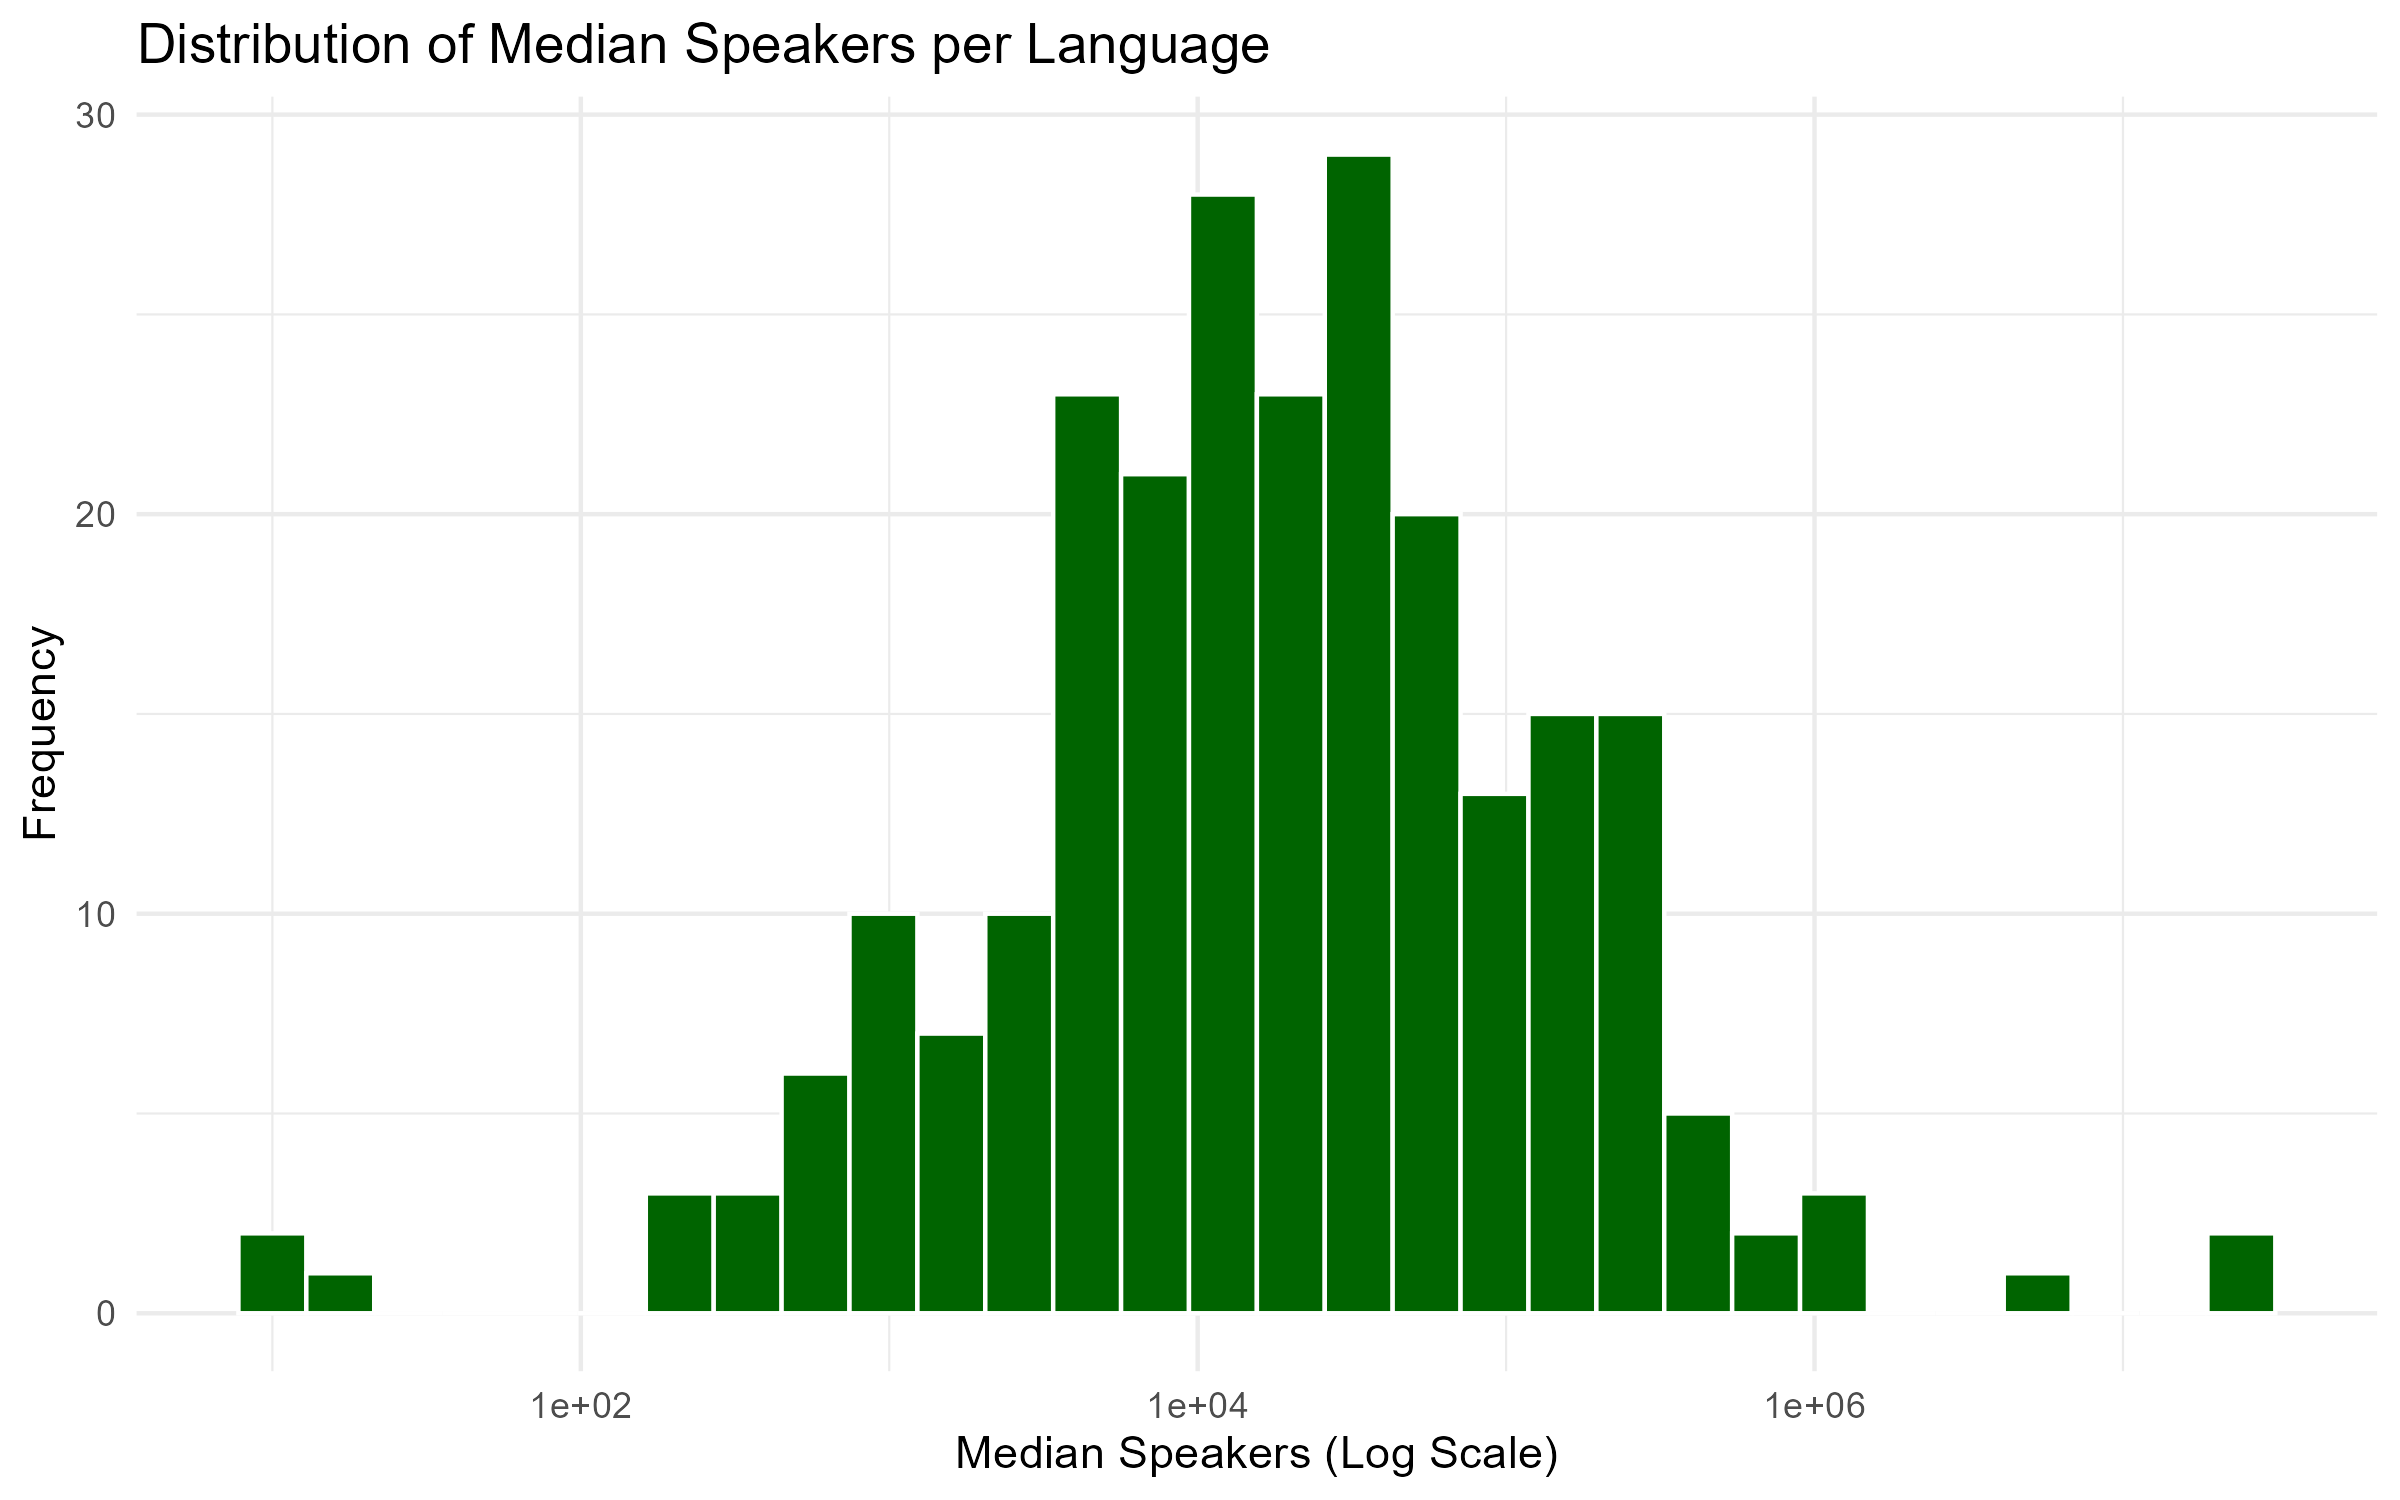
\includegraphics[width=0.8\textwidth]{PS6c_Dlamini.png}
\caption{Distribution of median number of speakers per language (log scale)}
\end{figure}
This histogram represents the distribution of the median number of speakers of each language per country, broken down by logarithmic scale. The distribution is highly skewed meaning that the number of speakers of most languages is relatively low but there are few languages that have large populations of speakers. This will help demonstrate the unequal sizes of the languages and emphasize the fact that the majority of languages are spoken by minor groups.

\end{document}
